\documentclass[10pt,fleqn]{beamer}

\usepackage[portuges,brazilian]{babel}
\usepackage[T1]{fontenc}
\usepackage[utf8]{inputenc}

\usepackage{multirow} % To merge cels horizontaly

\usepackage{multicol} % para utilizar ambiente "multicols"
\usepackage{pdfpages} % para incluir paginas de documentos PDFs
\usepackage{color, amsmath}
\usepackage{subfigure}
\usepackage{graphicx} % para incluir figuras
\usepackage[ruled,longend]{algorithm2e} % para escrever algoritmos
\usepackage{ulem}       % para trocar a fonte?

\usepackage{textcomp}
\usepackage{amssymb}

\graphicspath{{pics/}}

\definecolor{defblue}{rgb}{0.2, 0.2, 0.7}
\definecolor{defred}{rgb}{0.4, 0.0, 0.0}
\definecolor{defgreen}{rgb}{0.0, 0.4, 0.0}

\definecolor{ninfagreen}{rgb}{0.168, 0.541, 0.569} % changed this

% Set left ident of equations
\setlength{\mathindent}{4pt}

\newcommand{\mydef}[1]{{\vspace{8pt} \large \color{defblue} #1}}
\newcommand{\myred}[1]{{\bf \color{defred} #1}}
\newcommand{\mygreen}[1]{{\bf \color{defgreen} #1}}

\renewcommand{\rmdefault}{put} % Utopia Font
\renewcommand{\sfdefault}{put} % Utopia Font
\renewcommand{\emph}[1]{ {\bf #1} }

% Scale Equations
\newcommand*{\Scale}[2][4]{\scalebox{#1}{$#2$}}%

\newcommand{\litem}[1]{
  \item{#1 \vspace{9pt}}
}

%\usetheme{Berkeley}
%\usetheme{Hannover}
%\usetheme{Marcos}
%\usetheme{default}
\usetheme{Boadilla}
%\usetheme{Pittsburgh}

%\useinnertheme{rectangles}
%\useoutertheme{tree}
%\setbeamercolor{separation line}{use=structure,bg=structure.fg!50!bg}

%\usecolortheme{dolphin}
%\usecolortheme{seahorse}

\beamertemplatenavigationsymbolsempty

% Escrita dos algoritmos
\SetKwInput{KwIn}{Entrada}
\SetKwInput{KwOut}{Saída}
\SetKwFor{While}{enquanto}{faça:}{fim}
\SetKwFor{For}{para}{faça:}{fim}
\SetKwBlock{Begin}{início}{fim}
\SetKwIF{If}{ElseIf}{Else}{se}{então}{senão se}{senão}{fim}

\newcommand{\bigbullet}{\,\begin{picture}(-1,1)(-1,-2)\circle*{5}\end{picture}\ }
\newcommand{\termo}[1]{\textbf{#1}}
\newcommand{\titulo}[1]{\centering \LARGE \vfill \textcolor{defblue}{\textbf{#1}} \vfill }

\newcommand{\chamada}[1]{
  \textcolor{ninfagreen}{\textbf{#1}}
  \vspace{10pt}
}

%\title{Um Estudo da Eficiência da Autocentralidade no Problema de Isomorfismo de Grafos}
\title[]{Uma Análise Experimental de Métodos para Classificação Multirrótulo}
\subtitle{}
\author{Lucas Henrique Sousa Mello}
\institute[NINFA]{}
\date[Vitória, 17/03/2014]{Vitória, 17 de Março de 2014}
\subject{}

% Figura de fundo
\setbeamercolor{background canvas}{bg=white}
\setbeamertemplate{background}{
\includegraphics[width=\paperwidth,bb=0 0 1036 777]{fundo.png}}

% Posição dos títulos dos slides
\addtobeamertemplate{frametitle}{\vskip 2.5ex }{}
\addtobeamertemplate{frametitle}{\bf }{}

\begin{document}

\definecolor{beamer@blendedblue}{rgb}{0.168, 0.541, 0.569} % changed this

%\setbeamercolor{normal text}{fg=black,bg=white}
%\setbeamercolor{alerted text}{fg=red}
%\setbeamercolor{example text}{fg=green!50!black}

%\setbeamercolor{structure}{fg=beamer@blendedblue}

%\setbeamercolor{background canvas}{parent=normal text}
%\setbeamercolor{background}{parent=background canvas}

%\setbeamercolor{palette primary}{fg=yellow,bg=yellow} % changed this
%\setbeamercolor{palette secondary}{use=structure,fg=structure.fg!100!green} % changed this
%\setbeamercolor{palette tertiary}{use=structure,fg=structure.fg!100!green} % changed this

\begin{frame}
  \titlepage
\end{frame}

% \begin{frame}
%   \frametitle{Sumário}
%   \begin{itemize}
%     \litem{Introdução}
%     \litem{O problema da Mochila}
%     \litem{O Problema de Combate a Perdas}
%     \litem{Objetivos da Pesquisa}
%   \end{itemize}
% \end{frame}

\section{Introdução}

\begin{frame}
  \frametitle{Problemas de Classificação}
  \framesubtitle{O que são?}
  \begin{center}
  Determinar a classe de um objeto \\ dentre um conjunto pré-definido de classes. 
  \end{center}

  
  
  \begin{exampleblock}{Exemplos:}
  \begin{itemize}
   \item Fruta: descobrir se é Maçã, Uva ou Morango.
   \item Filme: descobrir se é de comédia ou não.
  \end{itemize}
  
 \end{exampleblock}
\end{frame}

\begin{frame}
  \frametitle{Problemas de Classificação}
  \framesubtitle{O que são?}
  
  Um objeto é descrito por um vetor de características.
  
    \begin{exampleblock}{Exemplo:}
  \begin{itemize}
   \item Fruta: Cor, massa e formato.
  \end{itemize}
  
 \end{exampleblock}
\end{frame}

\begin{frame}
  \frametitle{Problemas de Classificação Multirrótulo}
  \framesubtitle{O que são?}
  
  Um objeto pode estar associado a mais de uma classe simultaneamente.
  
    \begin{exampleblock}{Exemplo:}
  \begin{itemize}
   \item Filme: pode ser de comédia e romance.
  \end{itemize} 
  
 \end{exampleblock}
 Pode haver dependência entre as classes!
\end{frame}


\begin{frame}
  \frametitle{Problemas de Classificação Unirrótulo}
  \framesubtitle{O que são?}
  
  Seja $Y=\{r_1,r_2,r_3,...,r_m\}$ o conjunto dos $m$ possíveis rótulos.
%   \vspace{10pt}
  \begin{block}{Definição Formal:}
  \begin{align}
    \textrm{encontrar}
      \quad & f(x)=y \\
  	  \quad & \textrm{para todo }x \in X, \nonumber \\
  	  \quad & y\in Y
	  \nonumber
  \end{align}
  \end{block}
  
  Um classificador é $f$ aproximado.
  
\end{frame}


\begin{frame}
  \frametitle{Problemas de Classificação Multirrótulo}
  \framesubtitle{O que são?}
  
  Seja $Y=\{r_1,r_2,r_3,...,r_m\}$ o conjunto dos $m$ possíveis rótulos.
% %     \vspace{10pt}
  \begin{block}{Definição Formal:}
  \begin{align}
    \textrm{encontrar}
      \quad & f(x)=y \\
  	  \quad & \textrm{para todo }x \in X, \nonumber \\
  	  \quad & y\subseteq Y
	  \nonumber
  \end{align}
  \end{block}
  
  Um classificador é $f$ aproximado.
  
\end{frame}

%\begin{frame}
%  \frametitle{Otimização Contínua x Combinatória (Discreta)}
%  \begin{align*}
%    \textrm{maximizar}
%      \quad & z = f(x) & \textrm{maximizar} \quad & z = f(x) \\
%  	  \quad & x \in \mathbb{R} & \quad & x \in \mathbb{N} \\
%	  \nonumber
%  \end{align*}
%\end{frame}

\begin{frame}
  \frametitle{Problemas de Classificação}
  \framesubtitle{Complexidade}
  
  Temos $m$ possíveis rótulos.
  
  Número de possíveis saídas:
  \begin{itemize}
   \item Unirrótulo: $m$ (Linear)
   \item Multirrótulo: $2^m$ (Exponencial)
  \end{itemize}

\end{frame}

\begin{frame}
  \frametitle{Avaliação de Desempenho}
  Como estimar quão próximo o classificador ($\hat{f}$) é de $f$?
  
  \begin{itemize}
   \item Testes onde resultado esperado é conhecido.
   \begin{itemize}
    \item Para cada $x\in \{x_1,x_2,...,x_n\}$, $\hat{f}(x)=f(x)?$
   \end{itemize}

  \end{itemize}

\end{frame}

\begin{frame}
  \frametitle{Avaliação de Desempenho}
  \framesubtitle{Métricas Multirrótulo}
  Quão próximo cada teste de $\hat{f}(x)$ é de $f(x)$?
  \begin{center}
  $\{\textrm{Comédia,Romance}\} \approx \{\textrm{Comédia,Ação}\}$?
  \end{center}
  
  \begin{itemize}
  \litem{Subset Accuracy}: 1 se $\hat{f}(x)=f(x)$,~$0$~contrário.
  \litem{Hamming Loss}: $\frac{1}{m}(\hat{f}(x) \triangle f(x))$. 
  \litem{Example Based Accuracy}: \large{$\frac{|\hat{f}(x) \cap f(x)|}{|\hat{f}(x) \cup f(x)|}$}
  
  \end{itemize}
\end{frame}

\begin{frame}
  \frametitle{Avaliação de Desempenho}
  \framesubtitle{Métricas Multirrótulo}
  \begin{itemize}
  \litem{Subset Accuracy}: Confere se explorou dependência entre rótulos.
  \litem{Hamming Loss}: Confere se explorou as características.
  \litem{Example Based Accuracy}: Meio termo dos anteriores.
  \end{itemize}
  \begin{block}{}
Afirmações baseadas em argumentos matemáticos.
 \end{block}
 
\end{frame}

% CLASSIFICADORES MULTIRRÓTULOS: -------------------------------

\begin{frame}
  \frametitle{Classificadores Multirrótulo}
  \framesubtitle{Transformação do problema}
  
  Comumente é adotado a estratégia ``Dividir para Conquistar'':
    \begin{center}
  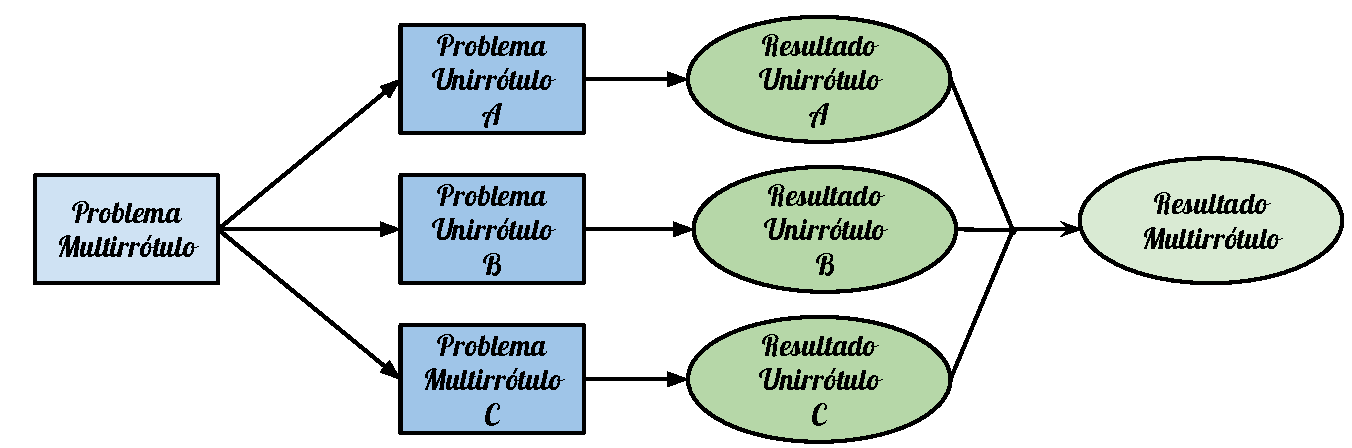
\includegraphics[scale=0.53]{transformar}
    \end{center}
\end{frame}

\begin{frame}
  \frametitle{Classificadores Multirrótulo}
  \framesubtitle{Binary Relevance}
  Fase de Treinamento do Binary Relevance (BR):
  
    \begin{center}
  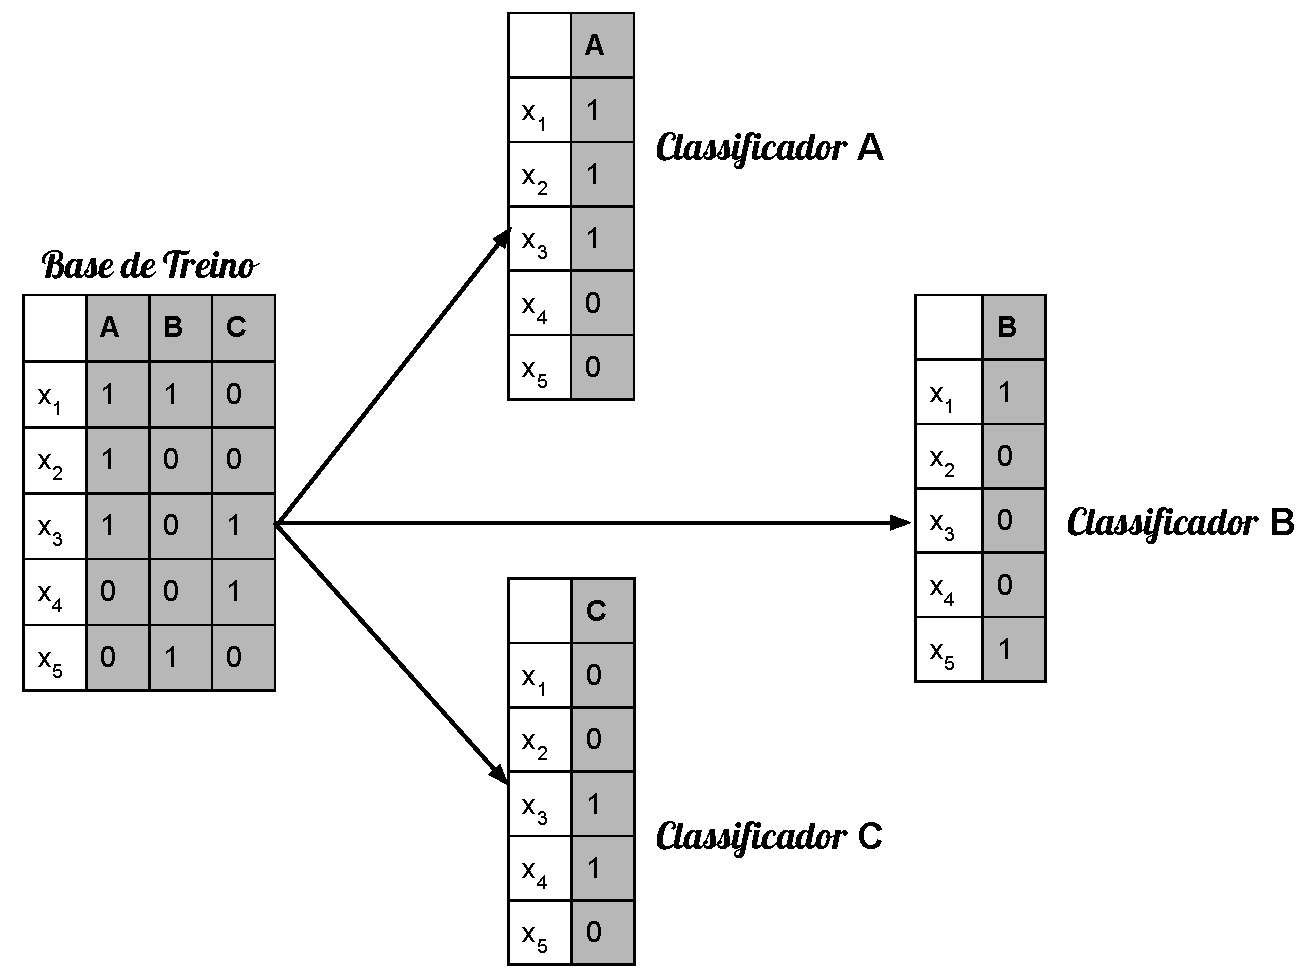
\includegraphics[scale=0.4]{BR-figure2}
    \end{center}
\end{frame}

\begin{frame}
  \frametitle{Classificadores Multirrótulo}
  \framesubtitle{Dependent Binary Relevance}
  
  O Dependent Binary Relevance (DBR) considera a dependência entre rótulos:
  
  \begin{itemize}
   \item É adicionado uma nova etapa ao BR.
%    \item Na nova etapa, rótulos são considerados características.
   \item Na nova etapa, rótulos são considerados características.
  \end{itemize}

\end{frame}

\begin{frame}
  \frametitle{Classificadores Multirrótulo}
  \framesubtitle{Dependent Binary Relevance}
  O Dependent Binary Relevance usa o BR:
  
    \begin{center}
  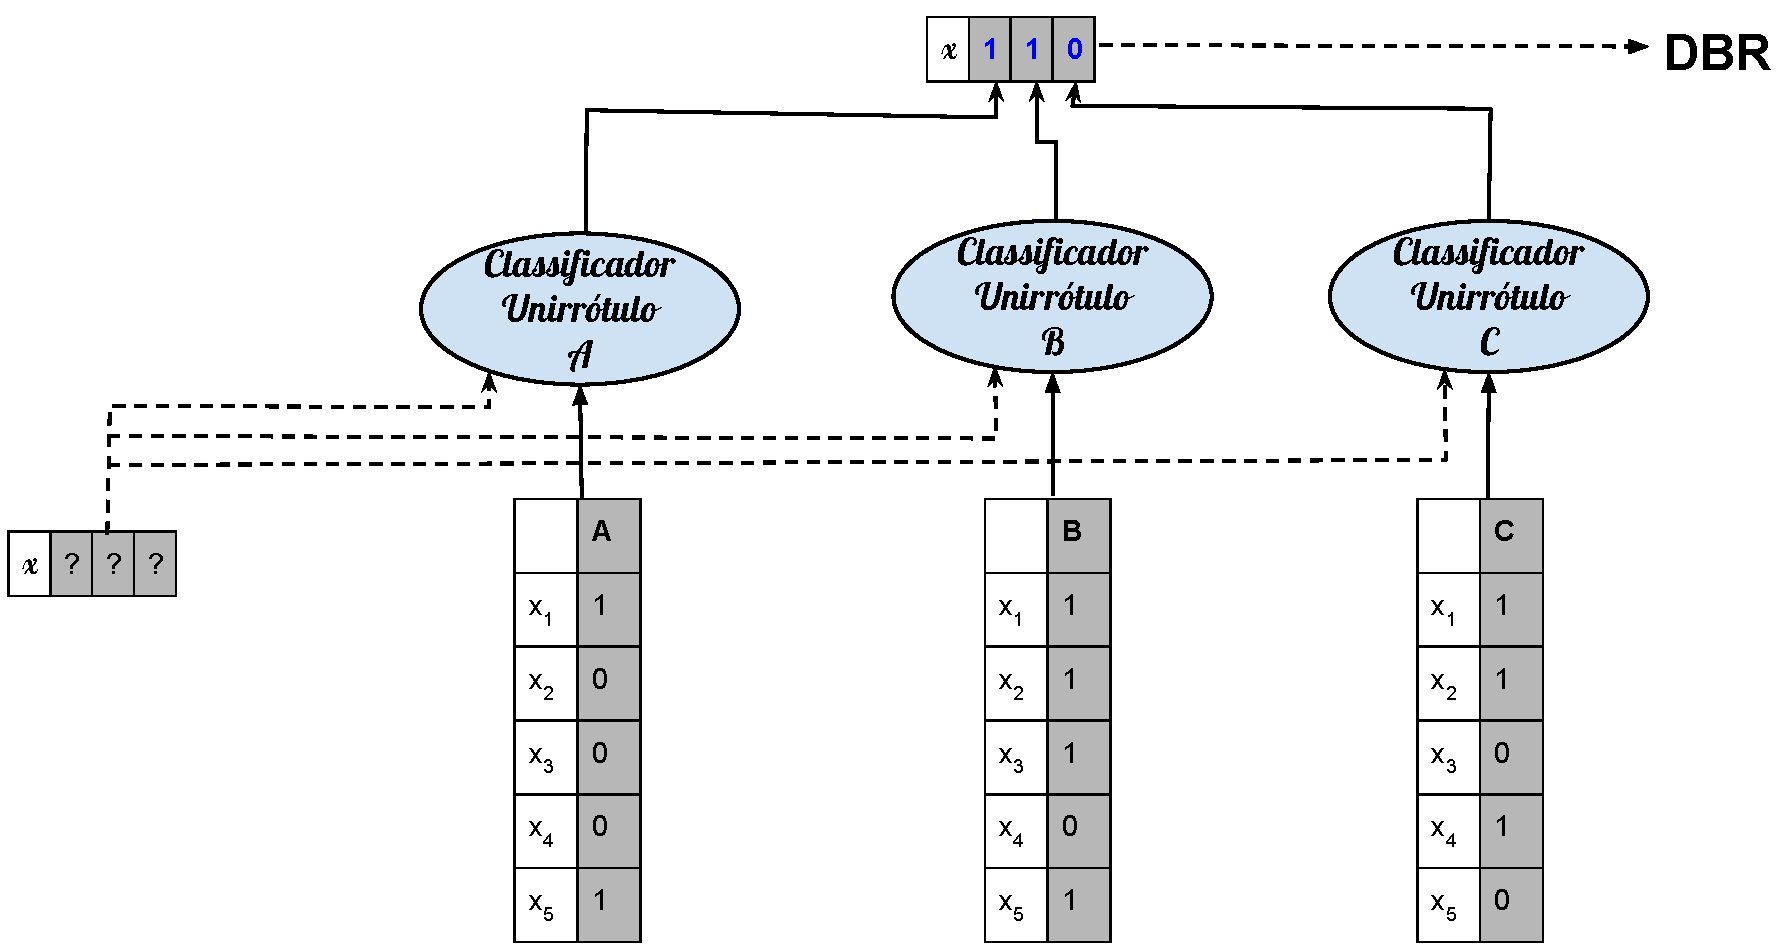
\includegraphics[scale=0.4]{DBR-prediction-fig}
    \end{center}
\end{frame}


\begin{frame}
  \frametitle{Classificadores Multirrótulo}
  \framesubtitle{Recursive Dependent Binary Relevance}
  O Recursive Dependent Binary Relevance (RDBR):
   \begin{itemize}
    \item Melhoria do DBR.
    \item Baseado no mesmo princípio: rótulos como boas características.
    \item Saída multirrótulo do DBR é reusado.
   \end{itemize}

\end{frame}

\begin{frame}
  \frametitle{Classificadores Multirrótulo}
  \framesubtitle{Recursive Dependent Binary Relevance}
    \begin{center}
  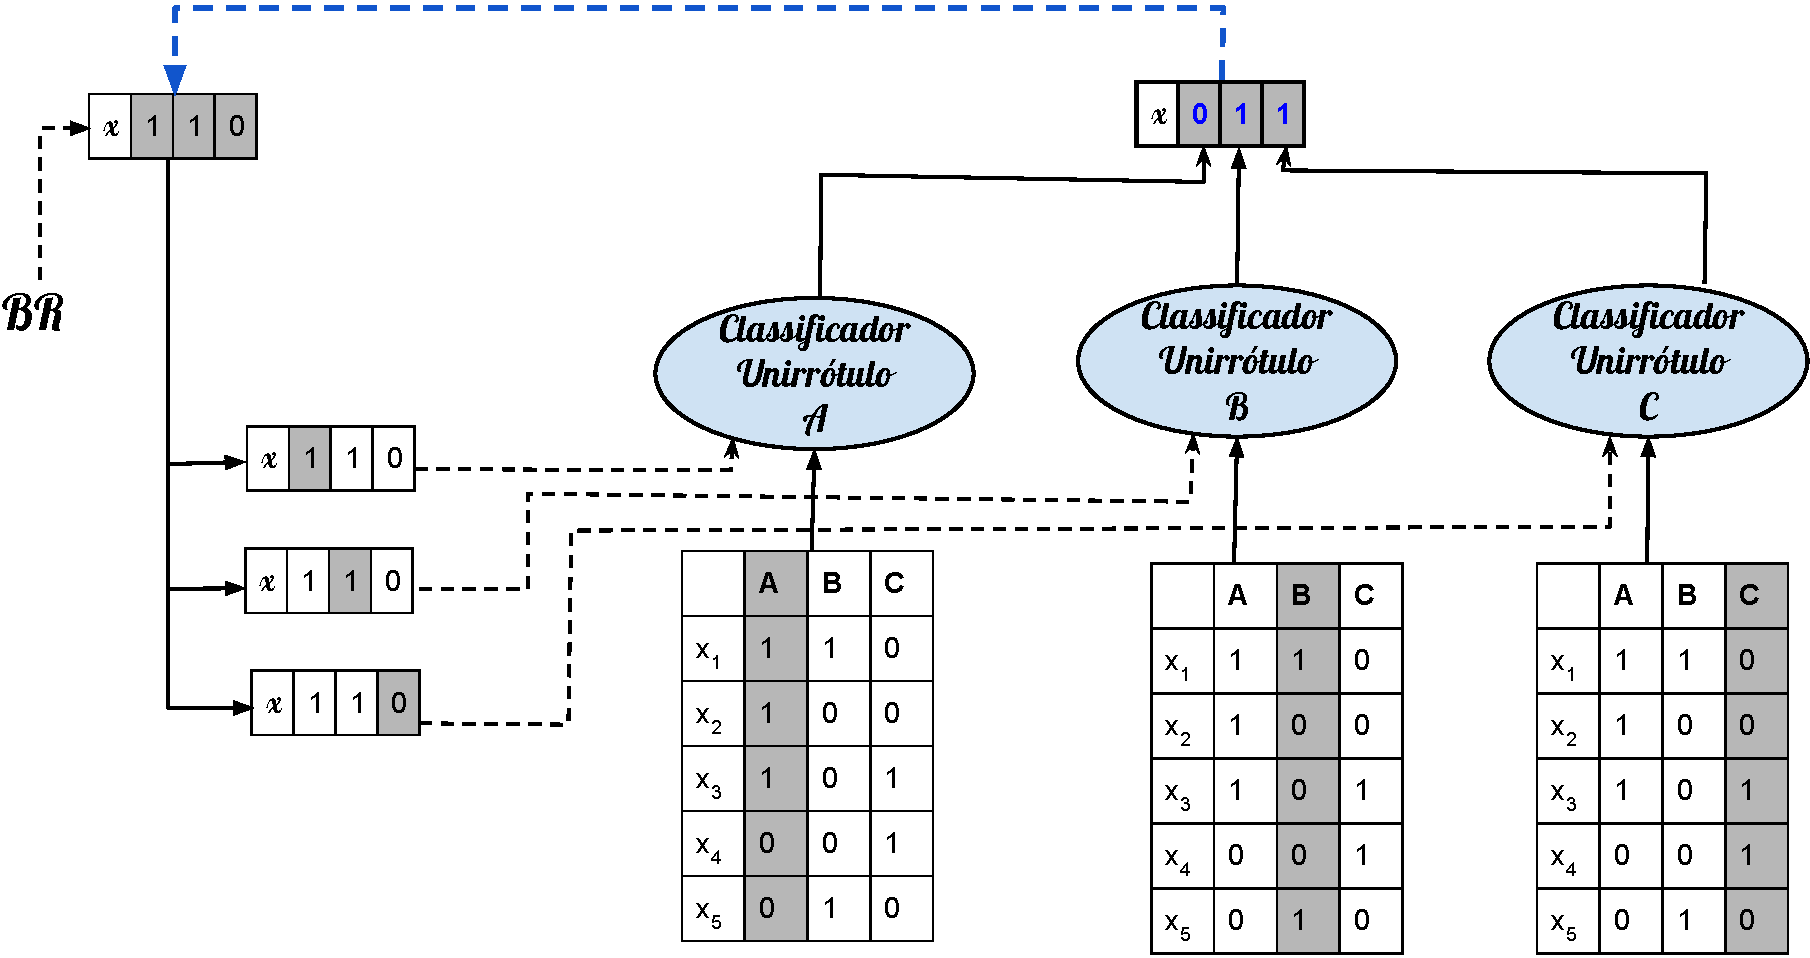
\includegraphics[scale=0.4]{RDBR-fig}
    \end{center}
\end{frame}

\begin{frame}
  \frametitle{Classificadores Multirrótulo}
  \framesubtitle{Recursive Dependent Binary Relevance}
    \begin{center}
  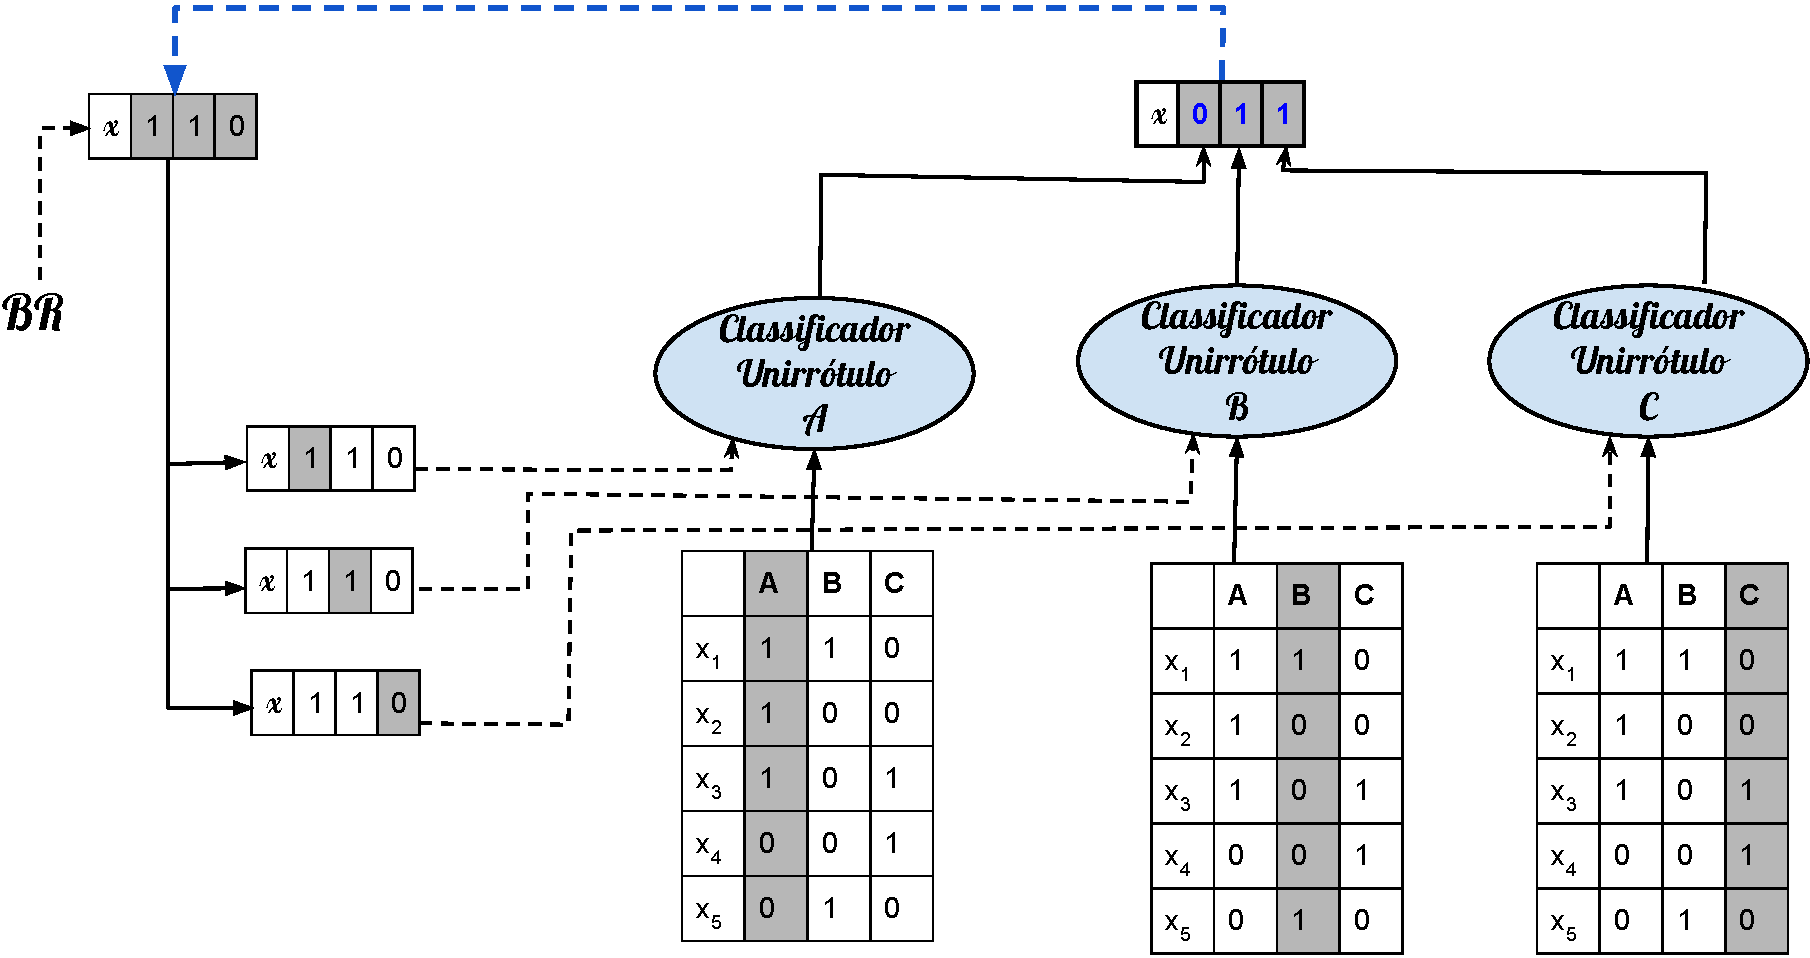
\includegraphics[scale=0.4]{RDBR-fig}
    \end{center}
\end{frame}

\begin{frame}
  \frametitle{Recursive Dependent Binary Relevance}
  \framesubtitle{Análise}
    
    Testes experimentais:
    \begin{itemize}
     \item 8 bases de dados
     \item 4 classificadores binários: KNN,SVM,Regressão Logística e C4.5.
     \item Validação Cruzada com 10 folds.
    \end{itemize}
    
    \begin{block}{Resultados}
     \begin{itemize}
      \item Melhorou em \textbf{80\%} dos testes;
      \item Empatou em \textbf{12.5\%};
      \item Piorou em \textbf{6.25\%}.
     \end{itemize}
    \end{block}
   \begin{center}
  $RDBR\geq DBR$, em \textbf{92.5\%} dos casos.
  \end{center}
\end{frame}

\begin{frame}
  \frametitle{Análise Empírica}
  \framesubtitle{Configuração Experimental}
  
    
\end{frame}  

\end{document}
